% Chapter Template

\chapter{Methodology} % Main chapter title

\label{Chapter4} % Change X to a consecutive number; for referencing this chapter elsewhere, use \ref{ChapterX}

\begin{figure}[h]
\centering
  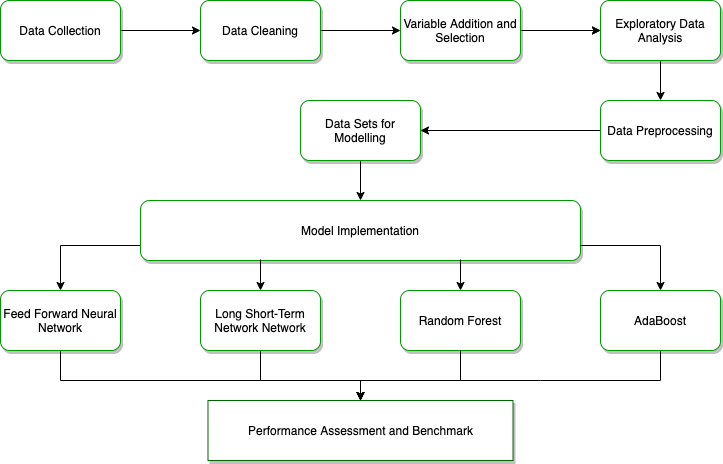
\includegraphics[scale =0.55]{/Users/pavansingh/Google Drive (UCT)/STA Honours/Project/Thesis/Write-Up/Draft/Figures/Methodprocess.png}
  \caption{Process of Comparative Analysis of Non-Linear Machine Learning Models}
  \label{}
\end{figure}


Our approach to this project begins by collecting the stock data. The collected data is then cleaned by checking for errors by examining day to day changes, null values or abnormalities (like negative prices) and missing values. We then proceeded onto variable selection for our models. Each model will be fed the same variables to ensure consistency and allow for a comparison of performance. Data preprocessing refers to analysing and transforming the input and output variables. This greatly assists the neural networks in learning the relevant patterns  (James, 2013). Since neural networks are pattern matchers, the representation of the data is critical in designing a successful network (Heaton \textit{et al.}, 2017). We then proceeded to generate training, testing and validation sets using our data set. Following this involved, selection of appropriate parameters and implementing the various models. 

%-----------------------------------
%	SUBSECTION 2
%-----------------------------------
\section{Neural Networks}

A simple artificial neural network (ANN) is typically organised into three sections: an input layer, a set of hidden layers, and an output layer - as shown in figure 4.2. The structure of ANN classifies into many types of architectures such as a Single layer, Feed-forward, and Recurrent networks (Agrwal \textit{et al.}, 2013). 

\begin{figure}[h]
\centering
  \includegraphics[scale =0.49]{/Users/pavansingh/Google Drive (UCT)/STA Honours/Project/Thesis/Python Coding/Figures/Methods/Untitled dwd.pdf}
  \caption{Simple Artificial Neural Network, with an input layer, a hidden layer and an output layer}
  \label{}
\end{figure}

Each layer of a simple ANN can contain one or more neurons. The first layer (input layer) is the layer connected to the input data. After that there could be one or more middle layers called hidden layers. The last layer is the output layer which shows the results (Agrwal \textit{et al.}, 2013).

The hidden and output layers are made up of a few interconnected nodes. These interconnected nodes contain an activation function which help the network learn complex patterns in the data (James, 2013). Hidden layers allow neural networks to perform non-linear mapping between the input and the output (Agrwal \textit{et al.}, 2013). Models can grow more deep by increasing the number of hidden layers and neurons in a given layer. This will also increase the mapping complexity (Heaton \textit{et al.}, 2017). The connections between neurons carry weights and some biases connected to each neuron. Simply, an ANN has weights associated with each input neuron and bias which also carries weight. An activation function is applied over the net input to calculate the output (Agrwal \textit{et al.}, 2013). The output is then compared to the target and weights are adjusted. 


A neural network is defined in terms of a recursive updating equation. To move forward through a network , called a forward pass, the network uses a formula 4.1 to calculate each neuron in the next layer. 

\begin{equation}
a^{(l)}=\sigma\left(W \boldsymbol{a}^{l-1}+\boldsymbol{b}\right)
\end{equation}

We note, neurons for activations $a$, weights $w$ and biases $b$ which are summed in vectors. This equation is responsible for taking us forward, until we get an output (Heaton \textit{et al.}, 2017). With that output $\hat{y}$, we can measure how good it is by using our cost function $C$ (4.2). We compare the $\hat{y}$ from our network with the result we wanted in the output layer $y$ (Heaton \textit{et al.}, 2017). This is done for every example in the data. The cost function which is commonly used for binary classification problems, and which is opted for in this paper, is called binary cross-entropy function (MSE):

\begin{equation}
\text {Binary Cross Entropy }=\frac{1}{N} \sum_{i=1}^{N}-\left(y_{i}{ }^{\star} \log \left(p_{i}\right)+\left(1-y_{i}\right)^{\star} \log \left(1-p_{i}\right)\right)
\end{equation}

Where, where $y$ is the label (1 or 0) and $p(y)$ is the predicted probability for label for all N points. It represents the average logarithmic error.

Now, we use our first result to go back and adjust the weights and biases. This is done so as to optimise the cost function - this is called a backwards pass (Heaton \textit{et al.}, 2017). Essentially, in the backward phase, we try to adjust the whole neural network, so that the output value is optimised (Heaton \textit{et al.}, 2017). We keep trying to optimise the cost function by running through new observations from our dataset. To update the network, we calculate gradients, which can be thought of as small updates to individual weights in each layer. The gradients are simply partial derivatives of the cost function, shown below:

\begin{equation}
\frac{\partial C}{\partial w^{(L)}}=\frac{\partial C}{\partial a^{(L)}} \frac{\partial a^{(L)}}{\partial z^{(L)}} \frac{\partial z^{(L)}}{\partial w^{(L)}} .
\end{equation}

%-----------------------------------
%	SUBSECTION 2
%-----------------------------------
\section{Feed-Forward Neural Network}

The architecture and process outlined in section 4.1 are representative of a multilayer perceptron neural network. It is the simplest form of an ANN, and is also the most popular type of neural network used (Gurney, 2018). In feedback networks, in contrast with recurrent networks (discussed next in section 4.3) all the connections are toward the output layer. The network structure for a feedforward neural network can be summarised by the updating equation 4.4.

\begin{equation}
a_{j}^{l}=\sigma_{l}\left(\sum_{k=1}^{d_{l-1}} a_{k}^{l-1} w_{k j}^{l}+b_{j}^{l}\right), \quad l=1,2, \ldots, L ; j=1,2, \ldots, d_{l}
\end{equation}

Where, 
\begin{itemize}
\item $\sigma_{l}(.)$ denotes an activation function on layer $l$ (e.g., sigmoid or hyperbolic tangent),
\item $d_{l-1}$ denotes the number of nodes in layer $l-1$ (the number of nodes in layer $l$ is $d_{l}$ ),
\item $w_{k j}^{l}$ denotes the $k j$-th weight parameter linking the $k$-th node in layer $l-1$ and $j$-th node in layer $l$ (although we transfer information from layer $l-1$ to layer $l$, we use the convention of indexing the weights using the superscript $l$-corresponding to the forward layer),
\item $b_{j}^{l}$ denotes the $j$-th bias in layer $l$,
\item and the equation is evaluated subject to the initial conditions $a_{j}^{(0)}=x_{i j}$ for all $j$ at the $i$-th training example (Pienaar, 2021)
\end{itemize}

There are many factors which should be discussed under the architecture of a neural network, apart from the weights, whose values cannot be estimated from the data - these are known as hyper-parameters. Before the learning process can begin, the value of a hyper-parameter must be determined.These include the number of input variables, the number of hidden layers and hidden nodes, the types of activation functions in the hidden and output layers and the value of the learning rate, amongst others (Agrwal \textit{et al.}, 2013). We outline the specific model specifications and architectures in chapter 5. 

With respect to the learning of the model, we are concerned with finding optimal hyper-parameters to fine to the model's complexity so as to control on the out-of-sample performance of the model. The hidden layer(s) provide the network with its ability to generalise. In theory, any continuous function may be approximated by a neural network with one hidden layer and a sufficient number of hidden neurons (Heaton \textit{et al.}, 2017). When we consider increasing the number of hidden layers, we need to also identify. the increased  computation time and increased risk of overfitting \footnote{Overfitting refers to the scenario where a model fits too closely - drawing too many characteristics - to the training data, and becomes unable to generalise well to unseen data.}. This can ultimately lead to poor out-of-sample forecasting performance. Few hidden nodes are usually recommended because there is less chance of overfitting (Agrwal \textit{et al.}, 2013). However, a neural network with too few nodes may not be able to learn the data's richness - leads to a model that under-fits the data. 

We also experiment with different optimisers and activation functions, so as to determine the appropriate model architecture and fit. Experimenting over the whole parameter space of all the parameters is beyond the scope of the paper. In this study, therefore, we focus on experimenting with the different values of key hyper-parameters, making use of a grid search. Grid search builds a model for every combination of hyper-parameters specified and evaluates each model (Gorr et al., 1994). 

%----------------------------------------------------------------------------------------
%	SUBSECTION 1
%----------------------------------------------------------------------------------------

\section{Long Short-Term Memory Neural Network}

\subsection{Overview of Recurrent Neural Networks}
A Recurrent Neural Network (RNN) is a class of Artificial Neural Network where connections between neurons form a directed cycle (Heaton \textit{et al.}, 2017).  In essence, these types of ANNs are designed in such a way to handle sequence dependence, as such, it has achieved great success in the field of sequence data (Che et al, 2015). Hence, RNNs in theory are perfectly suited for predicting movement of daily log returns of financial assets. According to Sak \textit{et al.} (2014), LSTM neural networks have outperformed the Deep Neural Networks (DNNs) and the simple RNN models for predicting the movements in stock data. 

A Simple RNN has a similar structure to the FFNN, but contains feedback connections (Che \textit{et al.}, 2018). That is, instead of having only neurons with connections from the input to the output, it also has neurons with connections from the output, again to the input. This is shown in equation 4.5. This additional connection can be used to store information over time providing the network with dynamic memory (Heaton \textit{et al.}, 2017). So, the current state of the network is a function its previous steps. Therefore, unlike feed-forward networks, they can use the information from the past to handle and predict sequential data. 

\begin{equation}
\begin{aligned}
h_{t} &=\tanh \left(\omega_{h} h_{t-1}+\omega_{x} x_{t}\right) \\
y_{t} &=\omega_{y} h_{t}
\end{aligned}
\end{equation}

where,

\begin{enumerate}
\item $x_{t}-$ input state
\item $y_{t}-$ output state
\item $h_{t}-$ current timestamp
\item $h_{t-1}-$ previous timestamp
\item $\omega_{h}-$ weight associated with the previous timestamp
\item $\omega_{x}-$ weight associated with the current input
\item $\omega_{y}-$ weight associated with the output
\end{enumerate}

\newpage
\subsection{Long Short-Term Memory Neural Networks}

LSTMs are a type of RNN, introduced by Schmidhuber in 1997, to overcome the vanishing gradient problem, which standard RNNs are susceptible to, by controlling the way information flows in the network (Schmidhuber, 1997). More precisely the model structure of an LSTM is defined so as to retain recurrence but to ensure that backpropagation does not degenerate in the practical sense. 

RNNs have have the property of being extremely deep, and after every iteration in the neural net, the data it holds gets vanished going deeper. LSTM does not use any activation function within its recurrent component. Thus thus the stored value is not iteratively modified. Hence the gradient does not tend to vanish when trained with backpropagation and thus resolves the gradient vanishing problem. 

\begin{figure}[h]
\centering
  \includegraphics[scale =0.65]{//Users/pavansingh/Google Drive (UCT)/STA Honours/Project/Thesis/Python Coding/Figures/Methods/sfasdf.pdf}
  \caption{LSTM Layer in Model.}
  \label{}
\end{figure}


LSTMs comprise of gates and a memory cell to analyse and process long term sequences such as time series. The network learns from both short term and long term memory. This is ensured, as the LASTM cell enforces a constant error flow through the designed cell state. The hidden layer is replaced by a complex block (see Figure 4.3). The complex block composed of computing units consisting of gates. These gates trap the error in the block. This structure makes the LSTM capable of learning long-term dependencies. 


The gates in the LSTM block include: 
\begin{itemize}
\item One forget gate which decides what information is going to be remembered/thrown away for the new state.
\item An input gate which determines which portion of a specific point in time is to be added.
\item An output gate that controls what is going to be the next output.
\item Sigmoid layer generates numbers between zero and one, describing how much of each component should be let through.
\item Tanh layer generates a new vector, which will be added to the state (Nelson \textit{et al.}, 2017).
\end{itemize}

\begin{figure}[h]
\centering
  \includegraphics[scale =0.951]{/Users/pavansingh/Google Drive (UCT)/STA Honours/Project/Thesis/Python Coding/Figures/Methods/sdssddd.pdf}
  \caption{LSTM forget gate.}
  \label{}
\end{figure}

The forget gate (see figure 4.4) takes the previous hidden state $h_{t-1}$ and current input $x_{t}$. Then by applying sigmoid function $\sigma$ returns output $f_{t}$ between 0 (forget) and 1 (keep). The output from the forget gate is multiplied with previous cell state $C_{t-1}$ to drop irrelevant information (Nelson \textit{et al.}, 2017).

\begin{equation}
f_{t}=\sigma\left(\omega_{f}\left[h_{t-1}, x_{t}\right]+b_{f}\right)
\end{equation}

\begin{figure}[h]
\centering
  \includegraphics[scale =0.951]{/Users/pavansingh/Google Drive (UCT)/STA Honours/Project/Thesis/Python Coding/Figures/Methods/sdsdsss.pdf}
  \caption{LSTM input gate.}
  \label{}
\end{figure}

The input gate (see figure 4.5) updates the cell state $C_{t}$ (Nelson \textit{et al.}, 2017). The sigmoid function $\sigma$ determines which values of previous hidden state $h_{t-1}$ and current input $x_{t}$ will be updated by returning the value $i_{t}$ between 0 (do not update) and 1 (update). Then the $\tanh$ gives weightage to the passed values and returns the level of importance $\tilde{C}_{t}$ ranging from $-1$ to 1, which also helps to regulate the network. Then $\tilde{C}_{t}$ is multiplied by $i_{t}$ which determines which outputs form $\tanh$ should be used to update the cell state $C_{t}$ (Nelson \textit{et al.}, 2017).

\begin{equation}
\begin{array}{l}
i_{t}=\sigma\left(\omega_{i}\left[h_{t-1}, x_{t}\right]+b_{i}\right) \\
\tilde{C}_{t}=\tanh \left(\omega_{c}\left[h_{t-1}, x_{t}\right]+b_{C}\right)
\end{array}
\end{equation}

\begin{figure}[h]
\centering
  \includegraphics[scale =0.951]{/Users/pavansingh/Google Drive (UCT)/STA Honours/Project/Thesis/Python Coding/Figures/Methods/wswsw.pdf}
  \caption{LSTM output gate.}
  \label{}
\end{figure}

Finally, the output gate (see figure 4.6) decides what the next hidden state should be (Nelson \textit{et al.}, 2017). It applies sigmoid function $\sigma$ to resolve which states to let through $o_{t}$ and $\tanh$ regularises the current cell state $C_{t}$. Multiplication of both outputs determines which information the hidden state should carry (Nelson \textit{et al.}, 2017).

The advantage of a LSTM network is that it can convey information gathered at an early stage and readily store it in memory for a long time, allowing for the generation of future long-distance dependencies as emphasised by Chung. J (2014). In contrast to a FFNN, in an LSTM network, each node is used as a memory cell that can store other information, whilst in a FFNN each node is a single activation function. 

Like any other neural network, an LSTM needs to be trained, so as to be able to learn the features of the modelled task and be able to predict. This process consists in computing the weights and biases of the LSTM by minimising an objective function, MSE, through some optimisation algorithms - we opted for SGD. Once the model is trained on the training set and validated on a validation set, it is then tested on a real out of sample testing. Finally, we note that our LSTM model is constructed as a supervised binary classification model, using 42 features, to predict the movement of three stocks. 


%-----------------------------------
%	SUBSECTION 2
%-----------------------------------

\section{Ensemble Decision Trees}

Decision trees are a type of machine learning technique that uses decision rules learned from training data to predict the value of a target variable. Each node in a decision tree represents a question leading to a yes-no answer for traversing the respective left and right nodes (Ampomah \textit{et al.}, 2020).



There are two groups of ensemble methods. These are usually identified depending on how they integrate the results for single ensemble prediction. 
\begin{itemize}
\item Averaging Methods: train several base estimators independently and then average their predictions (Ampomah \textit{et al.}, 2020). 
\item Boosting Methods: train base estimators sequentially with the specific goal to reduce the bias of the combined estimator (Ampomah \textit{et al.}, 2020).
\end{itemize}

The Random Forest and AdaBoost algorithms represent some of the most popular ensemble machine learning methods and are just extensions of the simple decision trees algorithm. 

\section{Random Forest}

For a variety of machine learning applications, decision trees can be used (Ampomah \textit{et al.}, 2020). However, trees that are grown deep to learn highly irregular patterns tend to overfit the training sets (Ampomah \textit{et al.}, 2020). Noise in the data, can lead to the tree to grow very differently, since decision trees inherently have low bias and high variance. Random Forest's overcome this problem, since it trains multiple decision trees using different combination of features. This is done at the cost of slightly increased bias. The multitude of multitude of decision trees are then merged together to obtain a more accurate prediction, as illustrated by figure 4.7. The Random Forest algorithm is summarised in the appendix B.

\begin{figure}[h]
\centering
  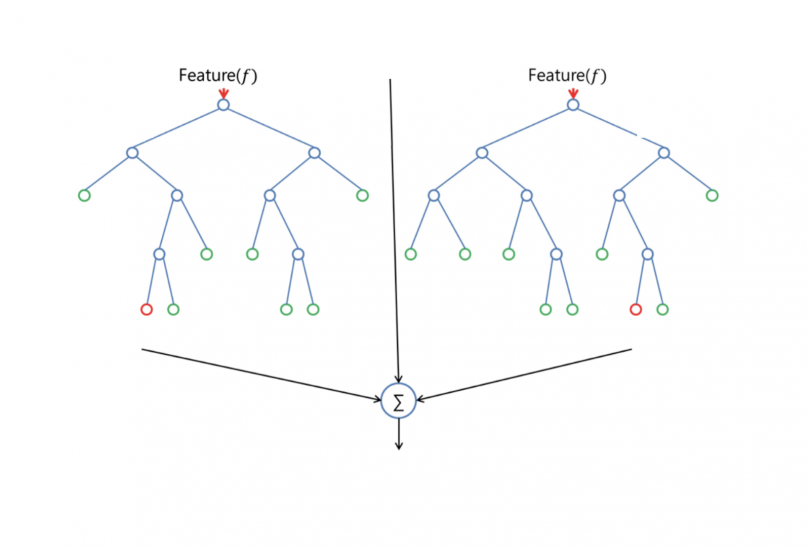
\includegraphics[scale =0.42]{/Users/pavansingh/Google Drive (UCT)/STA Honours/Project/Thesis/Write-Up/Draft/Figures/rf.png}
  \caption{Illustration of how Random Forests train multiple trees and then merge these trees to obtain a single prediction.}
  \label{}
\end{figure}

In a Random Forest, the data is recursively split into partitions. The tree makes use of recursive binary splitting to partition the feature space in such a way that the resulting residual sum of squares (RSS) is minimised at each step - for regression trees. Here RSS is the criterion for splitting at each node. The choice for the splitting criterion is based on some impurity measures such as Shannon Entropy or Gini impurity for classification problems. The approach is to choose the best splitting decision at a node such that reduction in impurity or RSS is as much as possible. 

In Random Forests, the goal of randomising the features in addition to the training observations is to further de-correlate the prediction errors of the individual trees. All features are not created equal, and a small number of highly relevant features will be selected much more frequently and earlier in the tree-construction process, making decision trees more alike across the ensemble. However, the less the generalisation errors of individual trees correlate, the more the overall variance will be reduced. 


%-----------------------------------
%	SUBSECTION 7
%-----------------------------------

\section{Adaptive Boosting}

\subsection{Boosting}
Boosting is another class of ensemble decision tree algorithms that involve combining the predictions from many weak learners (Ampomah \textit{et al.}, 2020). A weak learner is a model that is very simple, although has some skill on the data (Ampomah \textit{et al.}, 2020). This is done by building a model from the training data, then the subsequent models attempts to correct the errors from the previous model.

\begin{figure}[h]
\centering
  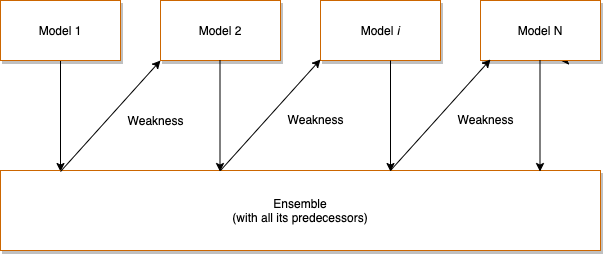
\includegraphics[scale =0.55]{/Users/pavansingh/Google Drive (UCT)/STA Honours/Project/Thesis/Write-Up/Draft/Figures/adaboost.png}
  \caption{Boosting algorithm for illustrated. The weakness depicts the errors. The subsequent models attempt to correct the errors from previous models. The models $1,2, 3,…, N$ are individual models that can be decision trees.}
  \label{}
\end{figure}

\subsection{AdaBoost Algorithm}

Adaptive boosting, or AdaBoost, is a type of boosting technique, which involves using very short (one-level) decision trees as weak learners that are added sequentially to the ensemble (Ampomah \textit{et al.}, 2020). 

AdaBoost is a significant departure from Random Forests, which builds ensembles of deep trees to reduce bias - there is no fixed depth in a random forest. AdaBoost, in contrast, grows shallow trees as weak learners - of depth 1. The algorithm only makes a node with two leaves, known as a stump. 

The algorithm starts with an equal-weighted training set and then successively alters the sample distribution (Ampomah \textit{et al.}, 2020). After each iteration, AdaBoost increases the weights of incorrectly classified observations and reduces the weights of correctly predicted samples so that subsequent weak learners focus more on particularly difficult cases. The process continues until a pre-set number of weak learners have been created (a user parameter) or no further improvement can be made on the training dataset. Once completed, you are left with a pool of weak learners each with a stage value. Once trained, the new decision tree is incorporated into the ensemble with a weight that reflects its contribution to reducing the training error (Ampomah \textit{et al.}, 2020). 

The process of Adaboost can be summarised as follows:
\begin{enumerate}
\item Creating the First Base Learner
\item Calculate the Total Error
\item Calculate Performance of the Stump
\item Update weights
\item Create a new data set 
\end{enumerate}



%-----------------------------------
%	SUBSECTION 5
%-----------------------------------

\section{ARIMA Model}


An Auto Regressive Integrated Moving Average, or ARIMA, is a class of time series models. An ARIMA model explains a given time series based on its own past values (lags and lagged forecast errors) so that it can be used to forecast future values (Zhang, 2003).The model is characterised by 3 parameters: $p$, $d$, $q$. The parameter $p$ is the order  of the auto regressive (AR) term. It refers to the number of lags of $Y$ to be used as predictors. While, $q$ is the order of the moving average (MA) term, which refers to the number of lagged forecast errors that should go into the ARIMA Model. and d is the number of differencing required to make the time series stationary. So ARIMA is essentially a time series method which combines terms of AR (autoregressive) and MA (moving average) (Zhang, 2003). 

The following equations depict ARIMA modelling:
$$
\begin{array}{l}
Y_{t}=\beta_{1} Y_{t-1}+\beta_{2} Y_{t-2}+\beta_{3} Y_{t-3}+\cdots+\beta_{0} Y_{0}+\varepsilon_{t} \\
Y_{t-1}=\beta_{1} Y_{t-2}+\beta_{2} Y_{t-3}+\cdots+\beta_{0} Y_{0}+\varepsilon_{t-1}
\end{array}

where, 
\begin{itemize}
\item Y_{t}=\text { function of lags of } Y_{t}$
\item $\beta_{t}=$ coefficient of the lag $t$ that model estimates
\item $\varepsilon_{t}=$ the errors from the equation (Zhang, 2003).
\end{itemize}


%-----------------------------------
%	SUBSECTION 6
%-----------------------------------

\section{Backpropagation}

Backpropagation revolutionised the landscape of machine learning with its introduction to neural networks in 1986 by Rumelhart \textit{et al.} (1986). Backpropagation is simply a way for a network to calculate the gradient of a loss function with respect to all the weights in the network. 
The expression for the partial derivative ($\frac{\partial C}{ \partial w}$) of the cost function $C$ with respect to any weight $w$ (or bias $b$ ) in the network, serves as the fundamental expression which allows for the gradients to calculated. When we adjust the weights and biases, the expression informs us how rapidly the cost changes. The method of backpropagation helps fine-tuning the weights of a neural network based on the error rate obtained in the previous iteration (Nelson \textit{et al.}, 2017).  Essentially, backpropagation method helps calculate the gradient of a loss function with respect to all the weights in the network. This plays a key role in the learning of the model. 

Backpropagation algorithm consists of 2 steps: 
\begin{enumerate}
\item Forward pass (feed forward) the values
\item Calculate the error and propagate it back to the earlier layers. 
\end{enumerate}

In this algorithm, the error between the actual output and target is propagated back to the hidden unit. For minimising the error, the weights are updated. To update the weights the error is calculated at the output layer . 

%-----------------------------------
%	SUBSECTION 2
%-----------------------------------
\section{Learning Algorithms and Training}

\subsection{Optimisers}

Optimisers is how the neural networks learn. In our neural network setup, we need an optimisation algorithm which best finds the value of the parameters (weights) that minimise the error when mapping inputs to outputs. There are several optimisers available, and the choice of optimiser can affect the accuracy of the models, as well as the speed of training (Rumelhart, 1995). Some of them include:

\begin{itemize}
\item Adam (adaptive moment estimation) 
\item RMSprop (root mean square propagation) 
\item SGD (stochastic gradient descent) 
\end{itemize}

Stochastic gradient descent (SGD) is an optimisation algorithm for minimising the loss of a predictive model with regard to a training dataset.More specifically, SGD is a form of gradient descent that works by using an iterative process to estimate the gradient towards minimising an objective loss function. The stochastic term comes about as samples are chosen at random. When lesser iterations are used, bigger steps are taken to reach the solution, and the model is said to have a high learning rate. Likewise, with more iterations, smaller steps are taken, resulting in a model with a small learning rate. 

In SGD, we take a batch of random sample and perform an update to weights and biases based on the average gradient from the batch. There exist many variations of stochastic gradient descent. 

Below is the equation 4.8 for SGD, which is used to update parameters in the neural networks. Equation 4.8 is used  to update the parameters of our network. This occurs in the backward pass. Backpropagation is used to calculate the gradient $\nabla$).

\begin{equation}
\theta=\theta-\eta \cdot \overbrace{\nabla_{\theta} C(\theta ; x, y)}^{\text {Backpropagation }}
\end{equation}

Where:
\begin{itemize}
\item $\theta$: a parameter. This can represent the weights, biases and activations. \item $\eta$ is the learning rate (eta)
\item $C$: cost function
\item $\nabla$: gradient (nabla), which is taken of $C$.
\item $\neta$: learning rate
\end{itemize}

Equation 4.8 indicates that we take each parameter theta $\theta$ and update it by taking the original parameter $\theta$ and subtract the learning rate $\eta$ times the ratio of change $\nabla C(\theta)$ (Agrwal \textit{et al.}, 2013).

\begin{figure}[h]
\centering
  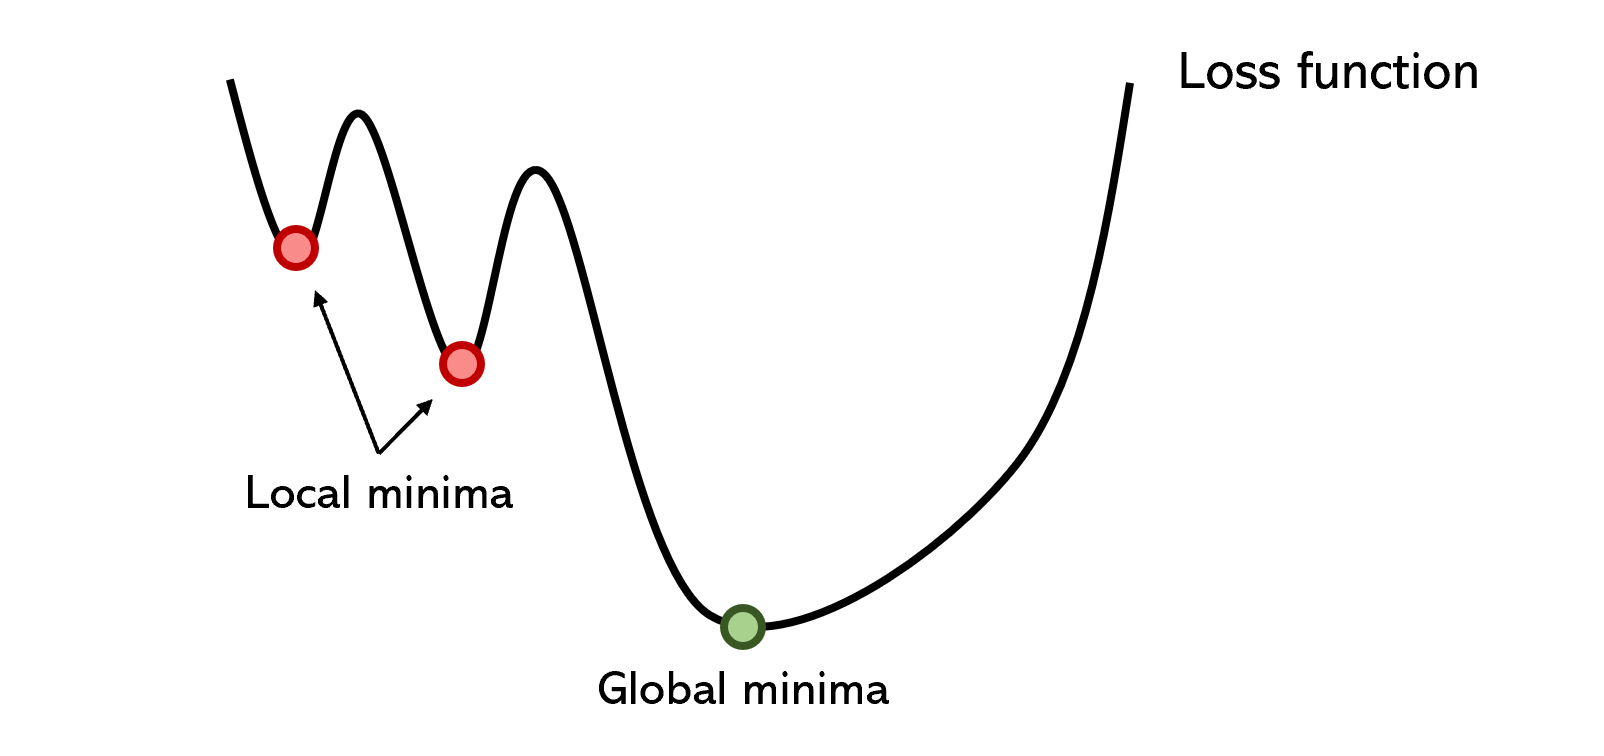
\includegraphics[scale =0.24]{/Users/pavansingh/Google Drive (UCT)/STA Honours/Project/Thesis/Write-Up/Draft/Figures/sgd.png}
  \caption{Stochastic Gradient Descent}
  \label{}
\end{figure}

The process of stochastic gradient descent can be summarised below:
\begin{enumerate}
\item Define a cost function
\item Start at a random point along the $x$-axis. Then the algorithm then looks to find a step to decrease the cost function most quickly
\item Calculate the gradient using backpropagation
\item Step in the opposite direction of the gradient. 
\end{enumerate}

The goal is to reach global minima (Agrwal \textit{et al.}, 2013).  However, often this is not possible. More often than not, we will find a local minima (see figure 4.9).

\subsection{Training}

Iteratively presenting examples of the correct known answers (targets) to a neural network, in order to learn patterns in the data is how a neural networks. trained. The goal of training is to try find the set of weights that. determine the global minima of the cost function (Heaton \textit{et al.}, 2017). For this paper, the training to testing data ratio has been kept as 95:5 in this paper. We achieve this by dividing the time series into three distinct sets called the training, testing, and validation (out-of-sample) sets (Heaton \textit{et al.}, 2017).  The training set is used to train the neural network to learn the underlying model form the data.  The validation set is used in our analysis to avoid overtraining of neural networks. And finally, our models are assessed on their predictive ability using the test set. 

\section{Activation Function}

An activation function is part of an artificial neuron that transforms the sum of weighted inputs into another value for the next layer (Heaton \textit{et al.}, 2017).  An artificial neuron is said to be activated when it passes a non-zero value to another neuron (Agrwal \textit{et al.}, 2013). There are several types of activation functions, some include:

\begin{itemize}
\item sigmoid
\item hyperbolic tangent (tanh)
\item rectified linear unit. (ReLU)
\item softmax
\end{itemize}


%-----------------------------------
%	SUBSECTION 7
%-----------------------------------

\section{Data}

The dataset used in this paper is Ford Motors, Google and Motorola Inc stock data scrapped from the Yahoo Finance Web site. Our data includes open price, close price, high price, low price and trading volume for the day. The data ranges from 2005 to 2015. We computed the log returns for the daily stocks for each company, according to the following equation:

\begin{equation}
\text{Log Daily Return} =  \log \left(\frac{\mathbf{P}_{\mathbf{d}}}{\mathbf{P}_{\mathbf{d - 1}}}\right)
\end{equation}
Where, $\mathrm{P}_{\mathrm{d}}$ : Closing Price for current day $\mathrm{d}$ and 
P $_{\mathrm{d}-1}:$ Closing Price of previous day $\mathrm{d}-1$.

Knowing which input variables are important for forecasting stock movements is pivotal. Although neural networks possess the ability to detect complex non-linear relationships among a number of different variables, however, for interpretability and reducing complexity, economic theory can greatly assist in choosing variables which are likely important predictors. We used the literature on trading and technical analysis, to guide us on which technical indicators and variables to use in our analysis. A popular approach, and one which we adopted, is to calculate various technical indicators which are based only on past prices (and occasionally volume and open price) of the market being forecasted. 

The dataset originally had six features, namely Open, High, Low, Close, Adjusted Close, Volume. The generated technical indicators were added later. The specific list of technical indicators and description of them can be found in appendix B.

An extract of the dataset for one stock (Ford Motors) used before the technical indicators were incorporated is shown in Table 4.1.

\begin{table}[h]
\centering
\begin{tabular}{lrrrrrr}
\toprule
{} &   Open &   High &    Low &  Close &  Adj Close &    Volume \\
Date       &        &        &        &        &            &           \\
\midrule
2005-01-03 &  14.66 &  14.75 &  14.51 &  14.71 &   9.271831 &   9852200 \\
2005-01-04 &  14.71 &  14.75 &  14.59 &  14.66 &   9.240314 &   9035400 \\
2005-01-05 &  14.63 &  14.66 &  14.42 &  14.43 &   9.095345 &  11376200 \\
2005-01-06 &  14.40 &  14.52 &  14.37 &  14.45 &   9.107951 &   6672600 \\
2005-01-07 &  14.48 &  14.65 &  14.45 &  14.65 &   9.234013 &  11452500 \\
\bottomrule
\end{tabular}
\caption{Extract of Data Set Before Adding Technical Indicators}
\end{table}

\begin{itemize}
\item Date : the date of the day on which the following trades were done
\item Open :  the price of a single stock at the opening of the market
 \item High : the highest price traded for the day
\item Low : the lowest price traded for the day
\item Close :  the price of the single stock at the closing of the market
\item Adjusted Close :  the adjusted closed price reflects the closing price of a given stock accounting for any corporate actions
\item Volume : refers to the amount of shares traded on that particular day
\end{itemize}

We also made sure to undertake data preprocessing, which refers to analysing and transforming the input and output variables to minimise noise, highlight important relationships, detect trends, and flatten the distribution of the variable to provide suitable input for our neural network models.

%-----------------------------------
%	SUBSECTION 8
%-----------------------------------

\section{Performance Criteria}

There are several measures of accuracy but each of them has advantages and limitations (Makridakis et al., 1983). As a result, none of them is commonly acknowledged as the best measurement. Hence, in our paper we make use of a number of performance measures to assess our models. Three measures are used to compare the forecasting accuracy of the models;  accuracy, F1 score. and AUC. All four models were assessed using these three metrics and the results were reported for each of the three stocks. The results can be summarised in a confusion matrix. A confusion matrix, or error matrix, is a square matrix that helps to visualise and describe the performance of a classification model for which the true values are known. We can extract the true positive and true negative metrics which can be used to compute the performance criteria. 

\begin{figure}[h]
\centering
  \includegraphics[scale =0.75]{/Users/pavansingh/Google Drive (UCT)/STA Honours/Project/Thesis/Python Coding/Figures/Methods/Untitled Diagram.pdf}
  \caption{Confusion Matrix}
  \label{}
\end{figure}

\subsection{Accuracy}
Accuracy is the quintessential classification metric (James, 2018). It is well suited for binary as well as a multi-class classification problem. Accuracy is the proportion of true results among the total number of cases examined. (Heaton \textit{et al.}, 2017). It summarises the performance of a respective model as the number of correct predictions divided by the total number of predictions. That is:

\begin{equation}
\text { Accuracy }=\frac{T P+T N}{T P+T N+F P+F N}
\end{equation}
Where $T P=$ True Positives, $T N=$ True Negatives, $F P=$ False Positives, and $F N$ = False Negatives.

\subsection{F1 Score}
Another metric we used, is the F1 Score. This measure is a number between 0 and 1 and is the harmonic mean of precision and recall (Nelson \textit{et al.}, 2017). Precision looks at what proportion of positive identifications was actually correct, while recall looks at what proportion of actual positives was identified correctly (Nelson \textit{et al.}, 2017). Since, the F1 score is the weighted average of Precision and Recall, this score takes both false positives and false negatives into account. An F1 score reaches its best value at 1 and worst value at 0. A low F1 score is an indication of both poor precision and poor recall. The formula of the F1 score is:

\begin{equation}
F_{1}=2 \cdot \frac{\text { precision } \cdot \text { recall }}{\text { precision }+\text { recall }}=\frac{\mathrm{TP}}{\mathrm{TP}+\frac{1}{2}(\mathrm{FP}+\mathrm{FN})}
\end{equation}

\subsection{AUC ROC}

The final measure we used is the AUC and ROC. This indicates how well the probabilities from the positive classes are separated from the negative classes. (Nelson \textit{et al.}, 2017). 

An ROC curve (receiver operating characteristic curve) is a graph showing the performance of a classification model at all classification thresholds (Nelson \textit{et al.}, 2017). This curve plots two parameters:
\begin{itemize}
\item True Positive Rate
\item False Positive Rate
\end{itemize}

More specifically the curve computes and plots all the combinations of true positive rates (TPR) and false positive rates (FPR) that result from producing predictions using any of the predicted scores as a threshold. The curve allows us to visualise, organise, and select classifiers based on their performance. A classifier that makes random predictions (taking into account class imbalance) will on average yield TPR and FPR that are equal so that the combinations will lie on the diagonal, which becomes the benchmark case.

The area under the curve (AUC) is defined as the area under the ROC plot that varies between 0.5 and the maximum of 1. It is a summary measure of how well the classifier's scores are able to rank data points with respect to their class membership. More specifically, the AUC of a classifier has the important statistical property of representing the probability that the classifier will rank a randomly chosen positive instance higher than a randomly chosen negative instance. In addition, the AUC has the benefit of not being sensitive to class imbalances. We opted for AUC since it Is scale-invariant and classification-threshold-invariant. That is, it measures how well predictions are ranked, rather than their absolute value. 

